\documentclass[11pt,a4paper]{article}

% Typeface: XeLaTeX with Latin Modern Roman (fontspec default)
\usepackage{fontspec}
\usepackage{polyglossia}
\setdefaultlanguage[variant=british]{english}

% Page: the measures of the note template (A4, 11 pt, 4.5 cm side margins, header and page count)
\usepackage[a4paper,left=4.5cm,right=4.5cm,top=4.5cm,bottom=4.1cm,headheight=14pt,headsep=0.55cm,
  footskip=0.55cm]{geometry}
\linespread{0.946}
\usepackage{fancyhdr}
\usepackage{lastpage}
\pagestyle{fancy}
\fancyhf{}
\fancyhead[L]{\small\textbf{PROJECT NOTE} $|$ Coin flipping}
\fancyhead[R]{\small\textbf{Compiled on:} \notedate}
\fancyfoot[C]{\small\thepage\,/\,\pageref{LastPage}}
\renewcommand{\headrulewidth}{0.4pt}

\usepackage{microtype}
\usepackage{amsmath,amssymb}
\usepackage{booktabs,array,tabularx}
\usepackage{graphicx}
\usepackage{enumitem}
\setlist{noitemsep, topsep=3pt, leftmargin=*}
\usepackage{xcolor}
\definecolor{secblue}{HTML}{1F3A5F}
\definecolor{boxback}{HTML}{EEF2F6}
\definecolor{mark}{HTML}{9B2226}
\definecolor{hl}{HTML}{FFF36B}
\usepackage{titlesec}
\titleformat{\section}{\color{secblue}\bfseries\normalsize}{\thesection.}{0.4em}{}
\titlespacing*{\section}{0pt}{10pt}{4pt}
\usepackage[font=small,labelfont=bf,labelsep=period,skip=4pt]{caption}
\usepackage[bottom]{footmisc}

\setlength{\parindent}{0pt}
\setlength{\parskip}{5pt}
\setlength{\textfloatsep}{10pt}
\emergencystretch=3em

\newcommand{\notedate}{\number\day\space\ifcase\month\or January\or February\or March\or April\or May\or June\or
  July\or August\or September\or October\or November\or December\fi\space\number\year}

\newcommand{\Paths}{2{,}000}
\newcommand{\ShareNow}{5.1}
\newcommand{\ShareByThousand}{53.1}
\newcommand{\ShareByMax}{74.4}
\newcommand{\ShareByMaxSe}{1.0}
\newcommand{\RmsSlope}{-0.496}
\newcommand{\RmsOverSe}{1.009}
\newcommand{\LilFrom}{922}
\newcommand{\LilThreeSigma}{1.2\times 10^{39}}
\newcommand{\NBelowHalf}{1{,}904}
\newcommand{\SlopeHalf}{-0.500}
\newcommand{\NBelowTenth}{7{,}129}
\newcommand{\SlopeTenth}{-0.500}
\newcommand{\NBelowHundredth}{80{,}246}
\newcommand{\SlopeHundredth}{-0.499}
\newcommand{\DHalfThirty}{0.072}
\newcommand{\DccHalfThirty}{$9.2\times 10^{-4}$}
\newcommand{\DHalfThousand}{0.0126}
\newcommand{\DccHalfThousand}{$2.7\times 10^{-5}$}
\newcommand{\DccHalfTenThousand}{$2.7\times 10^{-6}$}
\newcommand{\DccRatioHalf}{10.0}
\newcommand{\DccRatioTenth}{3.16}
\newcommand{\DRootNHalf}{0.3989}
\newcommand{\DHundredthThirty}{0.45}
\newcommand{\BeOverDHalf}{1.19}
\newcommand{\BeOverDHundredth}{1.78}
\newcommand{\HistN}{30}
\newcommand{\HistM}{20{,}000}
\newcommand{\VoneBins}{72}
\newcommand{\VoneWidth}{0.0097}
\newcommand{\Spacing}{0.0333}
\newcommand{\VoneEmpty}{51}
\newcommand{\VoneMax}{15.3}
\newcommand{\LatticeMax}{4.45}
\newcommand{\ExactMax}{4.33}
\newcommand{\NormalPeak}{4.37}
\newcommand{\PeakRatio}{3.5}


\begin{document}


\vspace*{14pt}
\begin{tabular}{@{}p{2.35cm}@{}p{\dimexpr\textwidth-2.35cm}@{}}
\textbf{TITLE:} & \textbf{\large Coin tosses: what the running mean, the 95\% band and the normal approximation actually show}\\[3pt]
\textbf{SUBJECT:} & Aim, method and results of the analyses in version 2 of the \texttt{coin-flipping-exercise} repository\\[3pt]
\textbf{AUTHOR:} & Muhammed İkbal Yılmaz (myucanlar@gmail.com)
\end{tabular}

\vspace{8pt}
\vspace{12pt}

\section{Aim and scope}

Let $X_1, X_2, \dots$ be independent tosses of a coin, $X_i = 1$ (heads) with probability $p$, and let
$\hat p_n = \frac1n\sum_{i=1}^n X_i$ be the proportion of heads after $n$ tosses. Its standard error is
$\mathrm{SE}(n) = \sqrt{p(1-p)/n}$. Version 1 of this project illustrated two classical results with simulations: the law of
large numbers (LLN), by a running mean $\hat p_n$ drawn inside the band $p \pm 1.96\,\mathrm{SE}(n)$, and the central limit
theorem (CLT), by histograms of $\hat p_n$ over many repeated experiments with a normal curve on top. Both illustrations were
judged by eye. This note replaces each visual impression by a measured or exactly computed quantity and asks three questions:

\begin{enumerate}
  \item \textbf{What does the 95\% band around a running mean say?} In particular, should a single path stay inside it?
  \item \textbf{How many tosses does the normal approximation need,} and how does that depend on $p$ and on the continuity
  correction? The fair coin ($p = 0.5$) of version 1 is the most favourable case; $p = 0.1$ and $p = 0.01$ stand for the
  small proportions (rare events, low response rates) that are common in applied work.
  \item \textbf{Why did the histograms of version 1 look spiky,} and how should a sample proportion be binned?
\end{enumerate}

\section{Method}

\begin{itemize}
  \item \textbf{Simulation.} NumPy's default generator with fixed seeds. Running means are computed from integer head counts,
  so they are exact ratios. Each repeated experiment of $n$ tosses is drawn directly as a binomial count.
  \item \textbf{Exact computations.} The binomial distribution $S_n \sim \mathrm{Bin}(n,p)$ is computed in log space. The
  distance between the binomial and the normal distribution is the Kolmogorov distance
  $D_n = \sup_x \lvert P(S_n \le x) - \Phi\bigl((x-np)/\sigma_n\bigr)\rvert$, $\sigma_n = \sqrt{np(1-p)}$. Because the
  binomial CDF is a step function, the supremum is attained at one of its jumps, so $D_n$ is computed exactly by checking
  both sides of every jump. With the continuity correction, $P(S_n \le k)$ is approximated by $\Phi\bigl((k+0.5-np)/\sigma_n\bigr)$.
  \item \textbf{Bounds.} The Berry--Esseen inequality gives $D_n \le C\rho/(\sigma^3\sqrt n)$, where for one toss
  $\sigma^2 = pq$ and $\rho = E|X-p|^3 = pq(p^2+q^2)$, $q = 1-p$. We use the best published constant, $C < 0.4748$
  (Shevtsova, 2011). The law of the iterated logarithm (LIL; Khintchine, 1924, for coin tosses; Hartman and Wintner, 1941)
  states that $\limsup_n \lvert\hat p_n - p\rvert / \sqrt{2p(1-p)\log\log n/n} = 1$ with probability one.
  \item \textbf{Checks.} Ten unit tests compare the code with independent computations: the binomial probabilities with exact
  rational arithmetic, $D_n$ with a brute-force search over a fine grid, the running means with a plain loop.
\end{itemize}

\section{Analysis 1: The running mean and the pointwise band (Figure~\ref{fig:lln})}

\textbf{Why.} Version 1 drew one running mean inside the band $p \pm 1.96\,\mathrm{SE}(n)$, called it a 95\% band, and noted
that the path stays close to $p$. The band is pointwise: for each fixed $n$, $\hat p_n$ lies in it with probability about
95\%. A reader looking at a whole path, however, naturally reads it as a region the path should stay in. These are different
statements, and this analysis measures both.

\textbf{Method.} \Paths{} independent paths of $10^5$ fair-coin tosses. For each $n$: the share of paths outside the band at
$n$; the share of paths that have been outside at least once up to $n$; and the root mean square (RMS) of $\hat p_n - p$.

\textbf{How to read the figure.} Left: 20 of the paths with the band (black) and the LIL envelope (grey, dashed). Right: the
blue curve is the share outside at a given $n$, which should be near the red dotted 5\% line if the band is correct; the black
curve is the share that has left the band at some point.

\begin{figure}[h]
\centering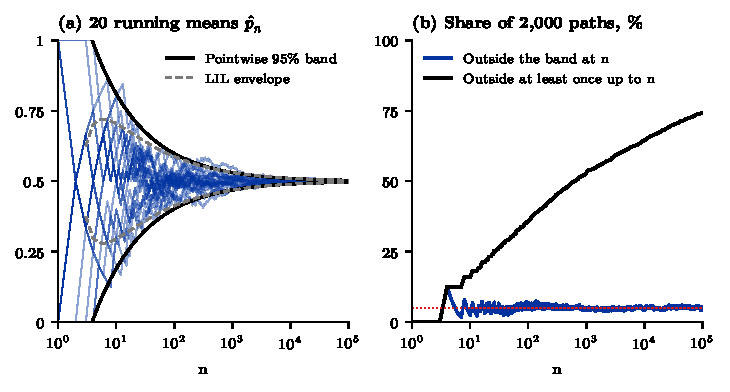
\includegraphics[width=\textwidth]{../figures/fig1_lln.pdf}
\caption{Left: running means of 20 fair-coin paths, the pointwise 95\% band and the LIL envelope. Right: share of \Paths{}
paths outside the band at $n$, and outside at least once up to $n$. Dotted: 5\%.}\label{fig:lln}
\end{figure}

\textbf{Finding.} The band is correct pointwise: for $10^3 \le n \le 10^5$ on average \ShareNow\% of paths are outside it at a
given $n$. But \ShareByThousand\% of paths have left it at least once by $n = 10^3$ and \ShareByMax\% by $n = 10^5$ (Monte Carlo
standard error \ShareByMaxSe{} percentage points), and the curve is still rising. This is what the LIL predicts: its envelope
is wider than the band for every $n \ge \LilFrom$ (where $\sqrt{2\log\log n} > 1.96$), so with probability one every path
leaves the band infinitely often, and the black curve tends to 100\%. The same holds for a $3\sigma$ band, but its envelope
crossing is at $n \approx \LilThreeSigma$, far beyond any simulation. The RMS error falls with slope $\RmsSlope$ on the
log--log scale and equals $\RmsOverSe\,\mathrm{SE}(n)$ at $n = 10^5$: the $1/\sqrt n$ rate of the LLN holds exactly as
predicted.

\textbf{Interpretation.} The band answers the question ``where is $\hat p_n$ likely to be for this $n$?'', not ``where will the
path stay?''. A path that leaves the band is not evidence against $p = 0.5$. Version 1's statement that the running mean is
``very close to 0.5'' by $n \approx 10^4$ can be made precise: at $n = 10^4$, $\mathrm{SE} = 0.005$, so $\hat p_n$ is within
$\pm 0.0098$ of $p$ with probability 95\% at that $n$. A band that holds for all $n$ at once has to be wider than the LIL
envelope for large $n$.

\section{Analysis 2: Accuracy of the normal approximation (Figure~\ref{fig:clt}, Table~\ref{tab:clt})}

\textbf{Why.} Version 1 judged the CLT from simulated histograms, which mixes the approximation error with simulation noise and
binning (see analysis 3). The distance between the binomial distribution and its normal approximation can be computed exactly,
and the Berry--Esseen bound says how large it can be. A common rule of thumb says that $n \ge 30$ is enough; the question is
whether the accuracy reached depends on $p$.

\textbf{Method.} For $p \in \{0.5, 0.1, 0.01\}$ and 46 values of $n$ between 5 and $10^5$, evenly spaced on a log scale: $D_n$
with and without continuity correction, and the Berry--Esseen bound.

\textbf{How to read the figure.} Both axes are logarithmic, so a quantity proportional to $n^{-1/2}$ is a line of slope
$-1/2$. Solid lines are exact distances, dashed lines the bounds of the same colour; the dotted line marks $D_n = 0.01$.

\begin{figure}[h]
\centering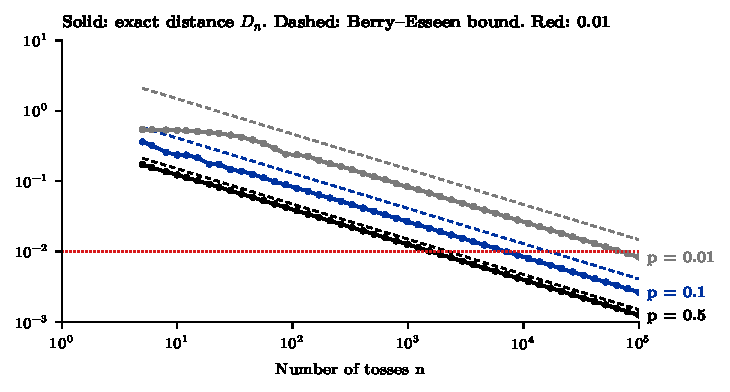
\includegraphics[width=\textwidth]{../figures/fig2_clt_accuracy.pdf}
\caption{Exact Kolmogorov distance between $\mathrm{Bin}(n,p)$ and its normal approximation (solid) and the Berry--Esseen
bound with $C = 0.4748$ (dashed). Dotted: $0.01$.}\label{fig:clt}
\end{figure}

\begin{table}[h]
\centering\footnotesize
\caption{Exact Kolmogorov distance $D_n$ without and with continuity correction (cc), and the first of the 46 values of $n$
from which $D_n$ stays below $0.01$.}\label{tab:clt}
\scriptsize\setlength{\tabcolsep}{1.7pt}
\begin{tabular}{@{}lrrrrrrrrr@{}}
\toprule
 & \multicolumn{2}{c}{$n = 30$} & \multicolumn{2}{c}{$n = 100$} & \multicolumn{2}{c}{$n = 1000$} & \multicolumn{2}{c}{$n = 10^4$} & $n$ for \\
\cmidrule(lr){2-3}\cmidrule(lr){4-5}\cmidrule(lr){6-7}\cmidrule(lr){8-9}
$p$ & $D_n$ & cc & $D_n$ & cc & $D_n$ & cc & $D_n$ & cc & $D_n < 0.01$ \\
\midrule
$0.5$ & 0.0722 & $9.2\times 10^{-4}$ & 0.0398 & $2.7\times 10^{-4}$ & 0.0126 & $2.7\times 10^{-5}$ & 0.00399 & $2.7\times 10^{-6}$ & 1{,}904 \\
$0.1$ & 0.147 & 0.0309 & 0.0832 & 0.0175 & 0.0266 & 0.00560 & 0.00842 & 0.00177 & 7{,}129 \\
$0.01$ & 0.449 & 0.0965 & 0.236 & 0.0584 & 0.0830 & 0.0204 & 0.0266 & 0.00654 & 80{,}246 \\
\bottomrule

\end{tabular}
\end{table}

\textbf{Finding.} For every $p$ the distance falls like $n^{-1/2}$ (slopes $\SlopeHalf$, $\SlopeTenth$, $\SlopeHundredth$ for
$n \ge 10^3$), as the Berry--Esseen inequality allows, and the bound is not loose: at $n = 1000$ it is \BeOverDHalf{} times the
exact distance for $p = 0.5$ and \BeOverDHundredth{} times for $p = 0.01$. For the fair coin, $\sqrt n\,D_n = \DRootNHalf$ at
$n = 10^4$, which is $1/\sqrt{2\pi} \approx 0.3989$: the error is half of the largest jump of the binomial CDF, which a
continuous curve cannot follow. The number of tosses needed depends strongly on $p$: $D_n$ stays below $0.01$ from
$n = \NBelowHalf$ for $p = 0.5$, $n = \NBelowTenth$ for $p = 0.1$ and $n = \NBelowHundredth$ for $p = 0.01$ (first values on
the grid). At $n = 30$ the distance is \DHalfThirty{} for $p = 0.5$ but \DHundredthThirty{} for $p = 0.01$. The continuity
correction removes the jump error: for $p = 0.5$ it reduces $D_{30}$ to \DccHalfThirty{}, and from $n = 1000$ to $10^4$ the
corrected distance falls by a factor \DccRatioHalf{}, i.e.\ like $1/n$. For $p = 0.1$ the corrected distance falls only by
\DccRatioTenth{} $\approx \sqrt{10}$: what remains comes from the skewness of the binomial distribution,
$(q-p)/\sqrt{npq}$, which is zero only for $p = 0.5$ and which no correction of a symmetric normal curve can remove.

\textbf{Interpretation.} ``$n \ge 30$'' is not a property of the CLT. How good the approximation is depends on $p$, through the
skewness, and on the accuracy needed. For a fair coin, the continuity correction makes the approximation very accurate already
at $n = 30$; for small proportions, exact binomial probabilities are the safer choice.

\section{Analysis 3: Histograms of a sample proportion (Figure~\ref{fig:hist})}

\textbf{Why.} Version 1 binned the simulated proportions with the Freedman--Diaconis rule, clipped to 25--160 bins. For small $n$
this rule produces tall, narrow spikes far above the normal curve (left panel of Figure~\ref{fig:hist}), which can be read as
a failure of the CLT. But
$\hat p_n$ is discrete: it takes only the $n+1$ values $k/n$.

\textbf{Method.} \HistM{} experiments of $n = \HistN$ fair-coin tosses (the setting of version 1 for $n = 30$), binned twice: with the version 1 rule, unchanged, and with
bins of width $1/n$ centred on the values $k/n$. On the right the exact probabilities $P(\hat p_n = k/n)$ are added, multiplied by
$n$ so that they are on the density scale of the histogram.

\textbf{How to read the figure.} Both panels show densities, so the total area of the bars is 1 in each. They share the vertical
axis, and the black curve is the same normal density in both.

\begin{figure}[h]
\centering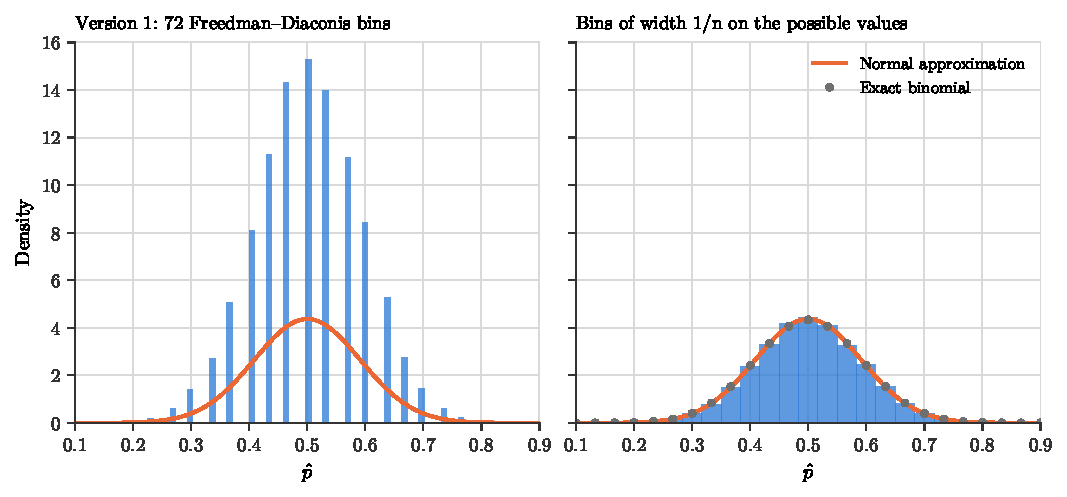
\includegraphics[width=\textwidth]{../figures/fig3_histogram.pdf}
\caption{\HistM{} sample proportions of $n = \HistN$ tosses. Left: the bins of version 1. Right: one bin of width $1/n$ per
possible value, with the exact binomial probabilities. Black: normal density with mean $0.5$ and variance $0.25/n$.}\label{fig:hist}
\end{figure}

\textbf{Finding.} The values of $\hat p_{30}$ are $1/30 = \Spacing$ apart, but the Freedman--Diaconis rule gives \VoneBins{} bins
of width \VoneWidth{}. Each possible value therefore falls into one narrow bin and the bins between values stay empty
(\VoneEmpty{} of \VoneBins{}). Because each bar is about a third as wide as the spacing, its height is about three times too
large: the tallest bar reaches \VoneMax{}, \PeakRatio{} times the peak of the normal density, \NormalPeak{}. With bins of width
$1/n$ the tallest bar is \LatticeMax{}, against \ExactMax{} for the exact probability and \NormalPeak{} for the normal density.

\textbf{Interpretation.} The spikes were an artefact of the binning, not a failure of the CLT. The Freedman--Diaconis rule is
derived for samples from a continuous density (Freedman and Diaconis, 1981); for discrete data the bin width should be a
multiple of the spacing of the possible values.

\section{Conclusions and limitations}

\begin{itemize}
  \item The pointwise 95\% band is correct at each $n$ but is not a region a path stays in: three quarters of the paths had left
  it by $n = 10^5$, and by the LIL every path leaves it infinitely often.
  \item The normal approximation to a proportion improves like $n^{-1/2}$, and the number of tosses it needs depends on $p$:
  from about $2{,}000$ to $80{,}000$ for $D_n < 0.01$ as $p$ goes from $0.5$ to $0.01$. The continuity correction removes most of
  the error for $p = 0.5$, much less for skewed cases.
  \item Histograms of discrete data need bins matched to the possible values; otherwise their shape says nothing about the CLT.
  \item Only independent tosses and three values of $p$ were studied. The Kolmogorov distance measures the largest error in a
  probability, not the relative error in the tails, which can be much larger. The thresholds for $D_n < 0.01$ are given on a
  grid of 46 values of $n$. Analysis 1 uses \Paths{} paths of length $10^5$.
\end{itemize}

\section*{References}
{\small
\setlength{\parskip}{2pt}
\hangindent=1.27cm\hangafter=1 Freedman, D., \& Diaconis, P. (1981). On the histogram as a density estimator: $L_2$ theory. \textit{Zeitschrift für
Wahrscheinlichkeitstheorie und verwandte Gebiete}, 57(4), 453--476.\par
\hangindent=1.27cm\hangafter=1 Hartman, P., \& Wintner, A. (1941). On the law of the iterated logarithm. \textit{American Journal of Mathematics}, 63(1), 169--176.\par
\hangindent=1.27cm\hangafter=1 Khintchine, A. (1924). Über einen Satz der Wahrscheinlichkeitsrechnung. \textit{Fundamenta Mathematicae}, 6, 9--20.\par
\hangindent=1.27cm\hangafter=1 Shevtsova, I. G. (2011). On the absolute constants in the Berry--Esseen type inequalities for identically distributed summands.
arXiv:1111.6554.\par
\hangindent=1.27cm\hangafter=1 NumPy documentation: \texttt{numpy.random.Generator}.\par

\smallskip
All numbers are generated from
\texttt{figures/*.csv} by \texttt{make\_paper.py}.
}

\end{document}
